\section{Architecture Integration}

\subsection{Model Support}

\begin{table}[H]
\centering
\small
\begin{tabular}{lllll}
\toprule
\textbf{Model} & \textbf{Attention path} & \textbf{Nested?} & \textbf{RoPE?} & \textbf{GQA?} \\
\midrule
DistilBERT & \texttt{layer[i].attention} & No & No & No \\
RoBERTa & \texttt{layer[i].attention.self} & Yes & No & No \\
GPT-2 & \texttt{h[i].attn} & No & No & No \\
Qwen3.5 & \texttt{layers[i].self\_attn} & No & Yes & Yes \\
\bottomrule
\end{tabular}
\end{table}

\subsection{Weight Extraction}

\subsubsection{UniversalAdapter First}

\begin{lstlisting}
from framework.core.adapters import UniversalAdapter
adapter = UniversalAdapter()
for k in ["q", "k", "v", "o"]:
    w, b = adapter.get\_weight\_bias(src, k)
\end{lstlisting}

\subsubsection{GPT-2 Fused Conv1D}

\begin{lstlisting}
c\_w = src.c\_attn.weight  # (in, out) for Conv1D
if c\_w.shape[0] \textless{} c\_w.shape[1]: c\_w = c\_w.t()
q\_w, k\_w, v\_w = c\_w.chunk(3, dim=0)
o\_w = src.c\_proj.weight.t()
\end{lstlisting}

\subsubsection{RoBERTa Nested}

\begin{lstlisting}
s = src.self
q\_w = s.query.weight
k\_w = s.key.weight
v\_w = s.value.weight
o\_w = src.output.dense.weight
\end{lstlisting}

\subsubsection{DistilBERT Flat}

\begin{lstlisting}
q\_w = src.q\_lin.weight
k\_w = src.k\_lin.weight
v\_w = src.v\_lin.weight
o\_w = src.out\_lin.weight
\end{lstlisting}

\subsection{Soft Fallback on Missing Weights}

Unlike SOA Fused Attention, we do \textbf{not} raise on missing weights. Instead:

\begin{lstlisting}
missing\_after = [k for k, (w, \_) in extracted.items() 
                 if w is None and (k != "o" or not self.is\_nested\_encoder)]
if missing\_after:
    logger.warning(f"Missing {missing\_after}, keeping Kaiming defaults.")
\end{lstlisting}

The projection retains its Kaiming initialization. This makes HymbaTransX 
more robust to unusual architectures but risks silent degradation.

\subsection{Second Query-Key Pair}

$W_{Q_2}, W_{K_2}$ are initialized via Kaiming uniform and \textbf{never copied} 
from the pretrained model -- the parent model has no analogue.

\begin{lstlisting}
nn.init.kaiming\_uniform\_(self.W\_q2.weight, a=math.sqrt(5))
nn.init.kaiming\_uniform\_(self.W\_k2.weight, a=math.sqrt(5))
\end{lstlisting}

\subsection{HeadRoPE Fallback}

If the parent model provides \texttt{position\_embeddings} (external RoPE), we use 
them directly. Otherwise, we apply \texttt{HeadRoPE}:

\begin{lstlisting}
if position\_embeddings is not None:
    cos, sin = position\_embeddings
    q1, k1 = apply\_rotary\_pos\_emb(q1, k1, cos, sin)
else:
    q1 = self.rope(q1)
    k1 = self.rope(k1)
\end{lstlisting}

\texttt{HeadRoPE} caches cos/sin tables up to 4096 tokens.

\subsection{Injection Algorithm}

\textbf{Algorithm 2:} Inject HymbaTransX into a model
\begin{lstlisting}
Input:  model M, config c
Output: M with attention replaced

1: layer\_list $\leftarrow$ find\_transformer\_layers(M)
2: for i, layer in enumerate(layer\_list):
3:     src $\leftarrow$ extract\_attention(layer)
4:     if src is None: continue
5:     try:
6:         new $\leftarrow$ HymbaTransXBlock(c, old\_attn=src)
7:         replace(layer, new)
8:     except Exception:
9:         log\_error("Layer {i} failed")
10: return M
\end{lstlisting}

\subsection{Nested Encoder Handling}

For RoBERTa, we set \texttt{is\_nested\_encoder = True}. The forward pass returns 
raw context, and the outer \texttt{output.dense} applies the projection.

\subsection{Causality Preservation}

\begin{lstlisting}
if self.is\_decoder:
    causal\_mask = torch.tril(torch.ones(L, L, dtype=torch.bool))
    scores1 = scores1.masked\_fill(~causal\_mask, -1e4)
    scores2 = scores2.masked\_fill(~causal\_mask, -1e4)
\end{lstlisting}

The mask applies to \textbf{both} attention maps before the subtraction.

\subsection{Cross-Attention}

Cross-attention raises \texttt{NotImplementedError}. HymbaTransX is encoder-only or 
decoder-only, not encoder-decoder.

\subsection{Registry}

\begin{lstlisting}
@ATTENTION\_REGISTRY.register("hymba\_transx")
class HymbaTransXBlock(BaseAttention):
    ...

@ATTENTION\_REGISTRY.register("hymba\_transx\_inject")
def inject\_hymba\_transx(...):
    ...
\end{lstlisting}
\begin{lstlisting}

---
\end{lstlisting}

\begin{figure}[H]
\centering
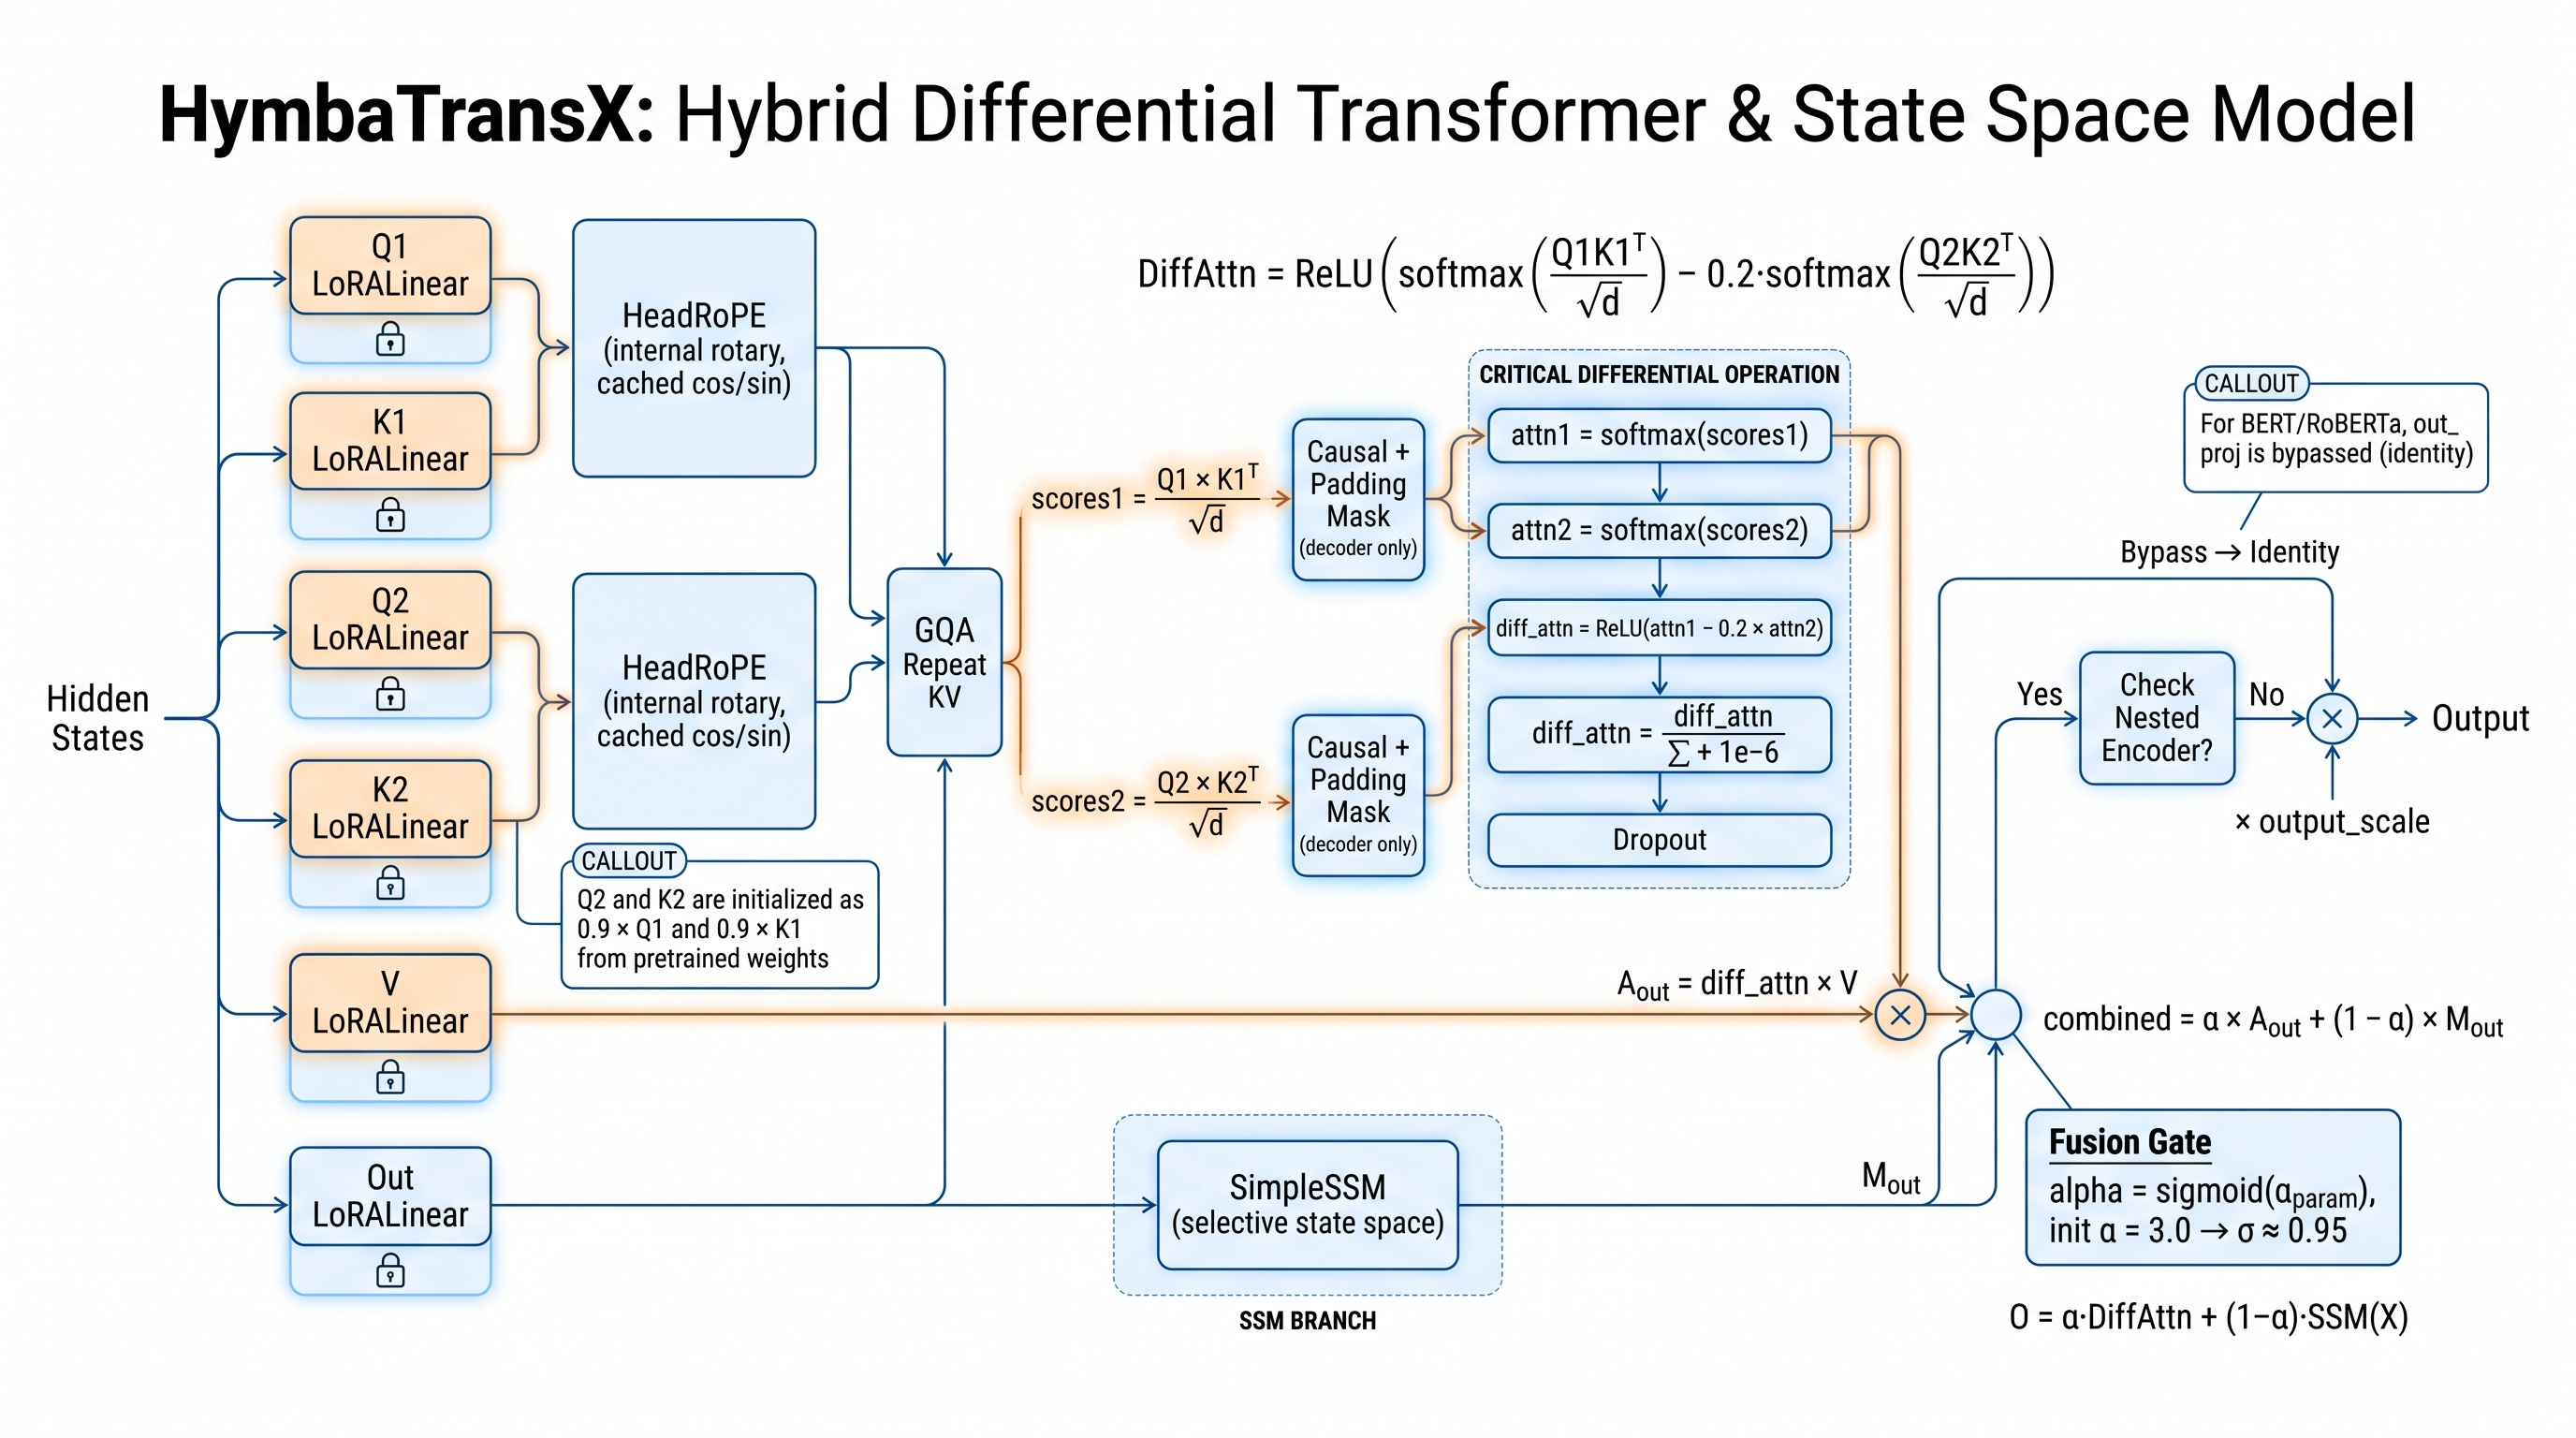
\includegraphics[width=\linewidth]{figures/architecture.jpeg}
\caption{High-level architectural diagram of hymba\_transx.}
\label{fig:arch\_hymba-transx}
\end{figure}

